%Hast du gut gemacht
% einleitung.tex -- Beispiel-File für die Einleitung
%
% (c) 2020 Prof Dr Andreas Müller, Hochschule Rapperswil
%
% !TEX root = ../../buch.tex
% !TEX encoding = UTF-8
\section{Gebietsunterteilung}
\label{parallelisierung:sec:Gebietsunterteilung}
\kopfrechts{Gebietsunterteilung}

\subsection{Motivation}
Wie im Kapitel der numerischen Methoden gezeigt, führt eine Verfeinerung der Raum- und Zeitauflösung zwar zu genaueren Ergebnissen, jedoch auch zu einem erheblich höheren Rechenaufwand. 
Mit zunehmender Gitterfeinheit steigt die Anzahl der Unbekannten quadratisch (in 2D) bzw. kubisch (in 3D).  
Um diese steigende Komplexität effizient bewältigen zu können, bietet sich die Methode der Gebietsunterteilung an.

Feldgleichungen wie die Wärmeleitungsgleichung besitzen eine lokale Struktur: 
der Wert in einem Gitterpunkt hängt nur von seinen direkten Nachbarn (räumlich und zeitlich) ab.  
Diese Eigenschaft erlaubt es, ein großes Problem in kleinere Teilprobleme zu zerlegen, sie getrennt zu berechnen und anschließend wieder zusammenzufügen.

\subsection{Mathematische Zerlegung}
Sei $\Omega \subset {R}^2$ das Gesamtgebiet, diskretisiert durch ein kartesisches Gitter.  
Wir zerlegen $\Omega$ in $P$ disjunkte Teilgebiete $\Omega_p$:
\begin{equation}
	\Omega = \bigcup_{p=1}^P \Omega_p,
	\qquad 
	\Omega_p \cap \Omega_q = \emptyset \quad \text{für } p \neq q.
\end{equation}

Das bedeutet:
\begin{itemize}
	\item Das Gesamtgebiet setzt sich vollständig aus den Teilgebieten zusammen.
	\item Jedes Gitterelement gehört genau zu einem Teilgebiet.
	\item Die Teilgebiete überlappen sich nicht, können sich aber an den Rändern berühren.
\end{itemize}

Anschaulich entspricht dies einem Puzzle: 
jedes Teilgebiet ist ein Puzzlestück, das nahtlos mit den Nachbarstücken zusammenpassen muss.

\subsection{Kopplungsbedingungen}
Damit die Zerlegung konsistent bleibt, müssen an den Schnittstellen (Rändern) bestimmte Bedingungen erfüllt sein:

\paragraph{Stetigkeit der Lösung.}
\begin{equation}
	T_{\Omega_p}(x,y,t) = T_{\Omega_q}(x,y,t)
	\qquad \forall (x,y) \in \partial \Omega_p \cap \partial \Omega_q.
\end{equation}
Die Temperatur darf an den Schnittkanten keine Sprünge zeigen.

\paragraph{Stetigkeit des Flusses.}
\begin{equation}
	- \kappa \, \nabla T_{\Omega_p} \cdot n
	=
	- \kappa \, \nabla T_{\Omega_q} \cdot n
	\qquad \forall (x,y) \in \partial \Omega_p \cap \partial \Omega_q.
\end{equation}
Es darf keine künstliche Wärmequelle oder -senke entstehen: der aus einem Gebiet austretende Fluss tritt ins Nachbargebiet ein.

\subsection{Diskrete Umsetzung mit Ghost-Zellen}
Betrachten wir die zweidimensionale Wärmeleitungsgleichung
\begin{equation}
	\frac{\partial T}{\partial t} = 
	\alpha \left(
	\frac{\partial^2 T}{\partial x^2} + \frac{\partial^2 T}{\partial y^2}
	\right).
\end{equation}
Mit FDM ergibt sich für ein quadratisches Gitter mit $\Delta x=\Delta y=\Delta l$ die Update-Formel:
\begin{equation}
	T_{i,j}^{n+1}
	=
	T_{i,j}^{n}
	+
	\lambda \left(
	T_{i+1,j}^{n}+T_{i-1,j}^{n}+T_{i,j+1}^{n}+T_{i,j-1}^{n}-4\,T_{i,j}^{n}
	\right),
	\quad
	\lambda=\frac{\alpha\Delta t}{(\Delta l)^2}.
	\label{eq:update-dd}
\end{equation}

Für innere Punkte eines Teilgebiets $\Omega_p$ kann \eqref{eq:update-dd} direkt berechnet werden.  
An Schnittkanten hingegen benötigt man Werte aus Nachbargebieten.  
Dazu führt man Ghost-Zellen ein:
\begin{itemize}
	\item Sie enthalten Kopien der Randwerte aus benachbarten Teilgebieten.
	\item Nach jedem Zeitschritt werden sie synchronisiert.
\end{itemize}
So kann jedes Teilgebiet lokal weiterrechnen. Dies erlaubt eine effiziente Parallelisierung, da nur die Schnittkanten kommuniziert werden müssen.

Abbildung \ref{parallelisierung:fig:ghostCells} illustriert beispielhaft diesen Datenaustausch über die Ränder verschiedener Teilgebiete mittels insgesamt 32 Ghost-Zellen an ausgewählten Stellen.

\begin{figure}[htbp]
	\centering
	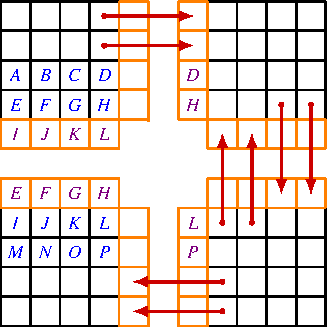
\includegraphics[width=0.6\textwidth]{papers/parallelisierung/images/ghostCells.pdf}
	\caption{Funktionsweise Ghost-Zellen}
	\label{parallelisierung:fig:ghostCells}
\end{figure}



\subsection{Speziallfall: Stationärer Grenzfall}
Für $n \to \infty$ strebt das Zeitschrittverfahren gegen ein stationäres Temperaturfeld. 
Dann verschwindet die Zeitableitung, und die Wärmeleitungsgleichung reduziert sich auf die Laplace-Gleichung
\[
\nabla^2 T = 0.
\]

Diskretisiert mit FDM erhält man für jeden inneren Gitterpunkt eine lineare Beziehung zu seinen Nachbarn:
\[
-4T_{i,j} + T_{i+1,j} + T_{i-1,j} + T_{i,j+1} + T_{i,j-1} = 0.
\]

Alle diese Gleichungen zusammen bilden ein lineares System
\[
\mathbf{A}\vec{u} = \vec{b}.
\]

\subsubsection{Beispiel: $5\times 5$-Gitter}

Einmal mehr legen wir uns ein Beispiel zurecht um dies besser zu verstehen. Dieses mal nehmen wir  ein $5\times 5$-Gitter mit folgenden Randwerten:
\[
T=100^\circ\mathrm{C}\ \text{(links)},\quad
T=0^\circ\mathrm{C}\ \text{(rechts)},\quad
T=80^\circ\mathrm{C}\ \text{(oben)},\quad
T=20^\circ\mathrm{C}\ \text{(unten)}.
\]

\begin{figure}[htbp]
	\centering
	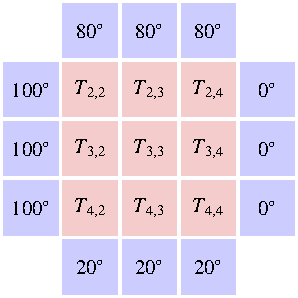
\includegraphics[width=0.6\textwidth]{papers/parallelisierung/images/stationaer.pdf}
	\caption{Beispiel Setup $5\times5$-Grid für stationären Grenzfall}
	\label{parallelisierung:fig:stationaer}
\end{figure}
Daraus ergeben sich $3\times 3 = 9$ innere Unbekannte.
Zusätzlich entfernen wir aus Gründen der Übersicht die Randzellen ohne Einfluss auf die inneren Zellen. Somit resultiert das Modell gemäss Abbildung \ref{parallelisierung:fig:stationaer}.


\subsubsection*{Diskretisierung}
Wenden wir nun die zuvor hergeleitete Explizite Updateformel \eqref{eq:update-dd} auf dieses Gitter an, resultieren die folgenden 9 Gleichungen:
\begin{alignat*}{6}
	-4\color{darkred}{T_{2,2}} &+ T_{3,2} &+ 80 &+ T_{2,3} &+ 100 &= 0, \\
	-4\color{darkred}{T_{2,3}} &+ T_{3,3} &+ 80 &+ T_{2,4} &+ T_{2,2} &= 0, \\
	-4\color{darkred}{T_{2,4}} &+ T_{3,4} &+ 80 &+ 0 &+ T_{2,3} &= 0, \\
	-4\color{darkred}{T_{3,2}} &+ T_{4,2} &+ T_{2,2} &+ T_{3,3} &+ 100 &= 0, \\
	-4\color{darkred}{T_{3,3}} &+ T_{4,3} &+ T_{2,3} &+ T_{3,4} &+ T_{3,2} &= 0, \\
	-4\color{darkred}{T_{3,4}} &+ T_{4,4} &+ T_{2,4} &+ 0 &+ T_{3,3} &= 0, \\
	-4\color{darkred}{T_{4,2}} &+ 20 &+ T_{3,2} &+ T_{4,3} &+ 100 &= 0, \\
	-4\color{darkred}{T_{4,3}} &+ 20 &+ T_{3,3} &+ T_{4,4} &+ T_{4,2} &= 0, \\
	-4\color{darkred}{T_{4,4}} &+ 20 &+ T_{3,4} &+ 0 &+ T_{4,3} &= 0.
\end{alignat*}

\subsubsection*{Matrixformulierung}
Wir ordnen die Unbekannten zeilenweise:
\[
\vec{u} =
\begin{bmatrix}
	T_{2,2}\\T_{2,3}\\T_{2,4}\\
	T_{3,2}\\T_{3,3}\\T_{3,4}\\
	T_{4,2}\\T_{4,3}\\T_{4,4}
\end{bmatrix}.
\]
Dann gilt:
\[
\mathbf{A}\vec{u}=\vec{b},
\]
mit
\[
\mathbf{A}=
\begin{bmatrix}
	-4& 1& 0& 1& 0& 0& 0& 0& 0\\
	1&-4& 1& 0& 1& 0& 0& 0& 0\\
	0& 1&-4& 0& 0& 1& 0& 0& 0\\
	1& 0& 0&-4& 1& 0& 1& 0& 0\\
	0& 1& 0& 1&-4& 1& 0& 1& 0\\
	0& 0& 1& 0& 1&-4& 0& 0& 1\\
	0& 0& 0& 1& 0& 0&-4& 1& 0\\
	0& 0& 0& 0& 1& 0& 1&-4& 1\\
	0& 0& 0& 0& 0& 1& 0& 1&-4
\end{bmatrix},
\quad
\vec{b}=
\begin{bmatrix}
	-180\\-80\\-80\\
	-100\\0\\0\\
	-120\\-20\\-20
\end{bmatrix}.
\]

\subsubsection*{Interpretation und Lösung}
\begin{itemize}
	\item $\mathbf{A}$ ist dünnbesetzt und spiegelt die 5-Punkt-Nachbarschaft wider.
	\item $\vec{b}$ enthält die Beiträge der Randwerte (verschieden je nach Position).
	\item Das System besitzt eine eindeutige Lösung: es liefert eine schräg verlaufende Temperaturverteilung zwischen den warmen und kalten Rändern.
\end{itemize}

\subsubsection*{Bemerkung zur Gebietsunterteilung im stationären Fall.}  
Im zeitabhängigen Fall werden Ghost-Zellen bei jedem Zeitschritt automatisch mit den Werten der Nachbargebiete gefüllt.  
Im stationären Fall dagegen gibt es keine Iteration in der Zeit, sodass die Ghost-Werte nicht direkt verfügbar sind.  
Um die Kopplung zwischen Subdomains herzustellen, gibt es zwei grundsätzliche Ansätze:

\begin{itemize}
	\item \emph{Algebraischer Ansatz:}  
	Das Gesamtsystem wird blockweise aufgestellt.  
	Die inneren Unbekannten jedes Teilgebiets bilden die Blöcke \(A_{pp}\), während die Kopplungen zu Nachbargebieten in den Randblöcken \(C_{pq}\) erscheinen.  
	Durch Verfahren wie das Schur-Komplement kann die Lösung des Gesamtsystems auf die Schnittkanten reduziert werden, wodurch die Rechenlast deutlich sinkt.  
	Weiterführende Details finden sich beispielsweise in \cite{parallelisierung:smith1996}.
	
	\item \emph{Iterative Ansätze:}  
	Domain-Decomposition-Verfahren berechnen die Teilgebiete wiederholt und tauschen dabei nach jeder Iteration die Werte an den Schnittkanten aus, bis Konsistenz erreicht ist.  
	
	Ein klassisches Beispiel ist die \emph{Schwarz-Methode}.  
	Hier werden an den künstlichen Rändern zwischen den Teilgebieten \emph{Dirichlet-Randbedingungen} vorgegeben, d.\,h.\ die benachbarten Teilgebiete liefern feste Temperaturwerte, die als Randwerte eingesetzt werden.  
	Genau diese Art von Randbedingungen haben wir auch im obigen Beispiel mit festen Temperaturen an den Außenrändern des Gitters verwendet.  
	Die Schwarz-Methode ist einfach und robust, kann jedoch bei vielen Teilgebieten langsam konvergieren.  
	Eine ausführliche Darstellung findet sich in \cite{parallelisierung:quarteroniValli1999}.  
	
	Eine leistungsfähigere Alternative ist die \emph{Neumann--Neumann-Methode}.  
	In diesem Verfahren werden an den Schnittkanten \emph{Neumann-Randbedingungen} eingesetzt, also Bedingungen für die Flüsse (z.\,B.\ Wärmeströme) über die Gebietsgrenzen hinweg.  
	Die Subdomänen werden parallel berechnet, und die Flusswerte an den Interfaces werden iterativ korrigiert, bis Konsistenz erreicht ist.  
	Dieser Ansatz eignet sich besonders für elliptische Probleme und skaliert gut auf parallelen Rechnerarchitekturen.  
	Details hierzu finden sich in \cite{parallelisierung:Gander}.
\end{itemize}


\subsection{Praktische Aspekte}

\subsubsection {Lastverteilung und Kommunikation.}
Die Kosten pro Zeitschritt sind proportional zur Anzahl der Gitterpunkte im Teilgebiet 
($\mathcal{O}(|\Omega_p|)$).  
Die Kommunikationskosten entstehen durch den Austausch von Ghost-Zellen und hängen von der Länge der Schnittkante ab.  
Für eine effiziente Parallelisierung ist es daher vorteilhaft, Teilgebiete mit möglichst kleinem 
Umfang/Flächen-Verhältnis zu wählen.  
In 2D bedeutet dies, dass quadratische Teilgebiete günstiger sind als lange, schmale Streifen.
Im 3D-Fall spricht man analog vom Oberflächen/Volumen-Verhältnis.  

\subsubsection {Stabilität.}
Die Stabilitätskriterien der expliziten Finite-Differenzen-Methode gelten auch bei der Gebietsunterteilung unverändert.  
Insbesondere muss in 2D für ein quadratisches Gitter stets
\[
\lambda = \frac{\alpha \Delta t}{(\Delta l)^2} \leq \tfrac{1}{4}
\]
gelten.  
Diese Bedingung ist lokal in jedem Teilgebiet genauso einzuhalten wie global.  



